\section{Implementation}
\begin{figure}[t!]
    \centering{}
	\subfloat[Architecture] { 
    	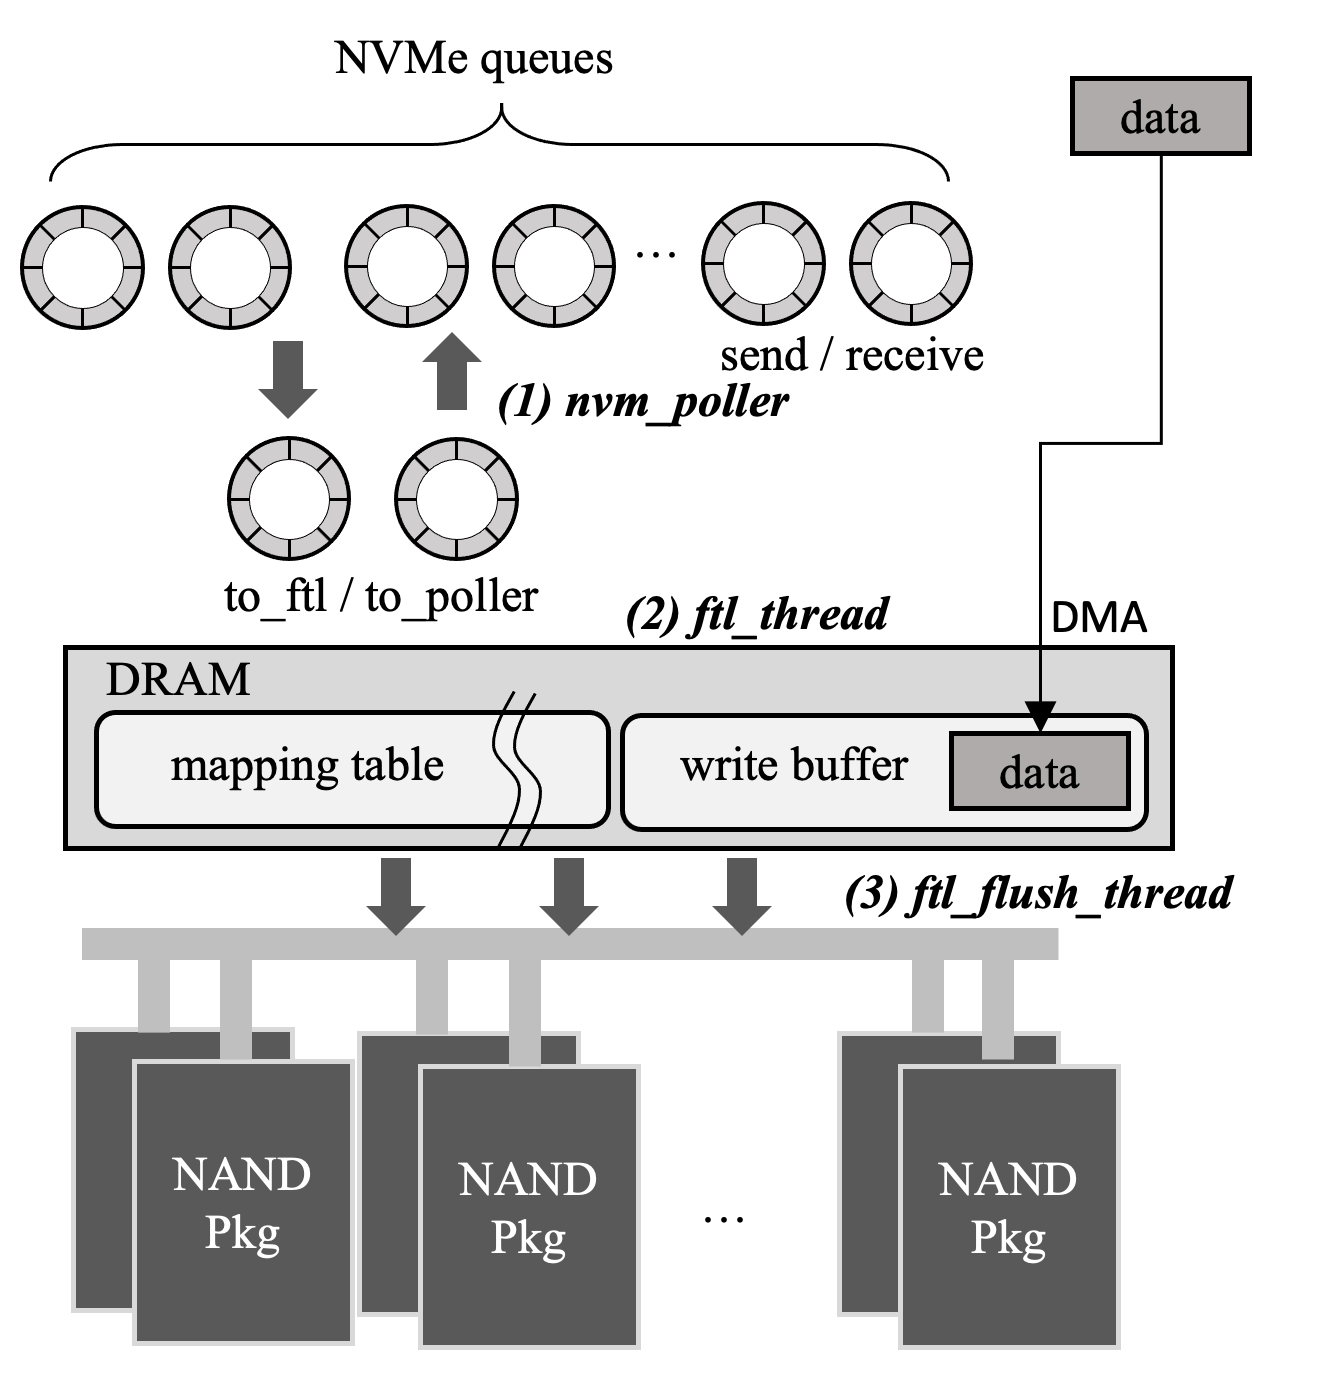
\includegraphics[width=0.3\textwidth]{figure/dawid_ssd_archi_new.eps}
	} \\
	\subfloat[Data structures for FTL]{ 
    	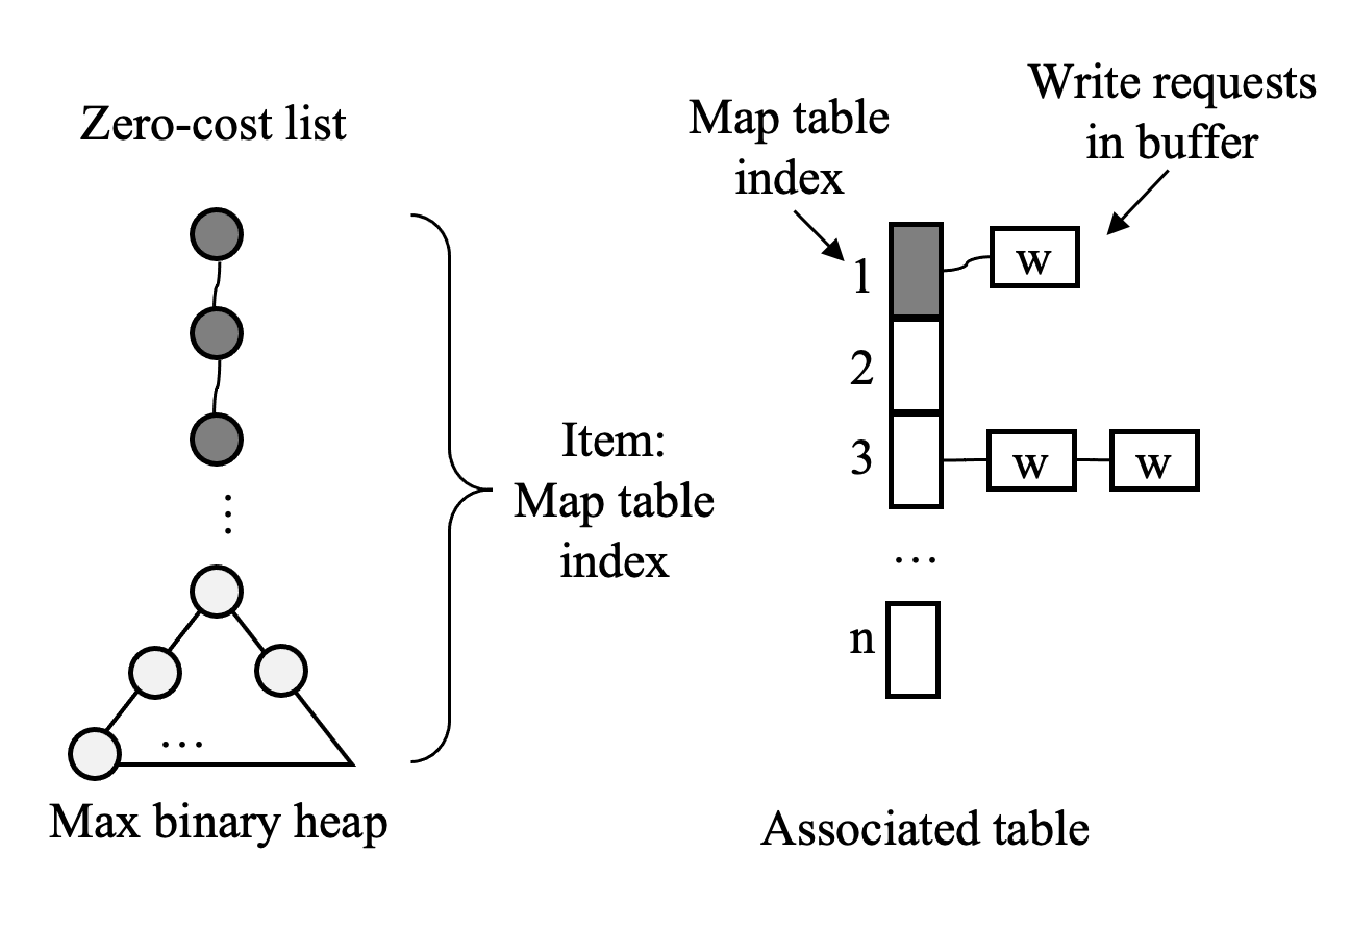
\includegraphics[width=0.4\textwidth]{figure/dawid_ds.eps}
	}

    %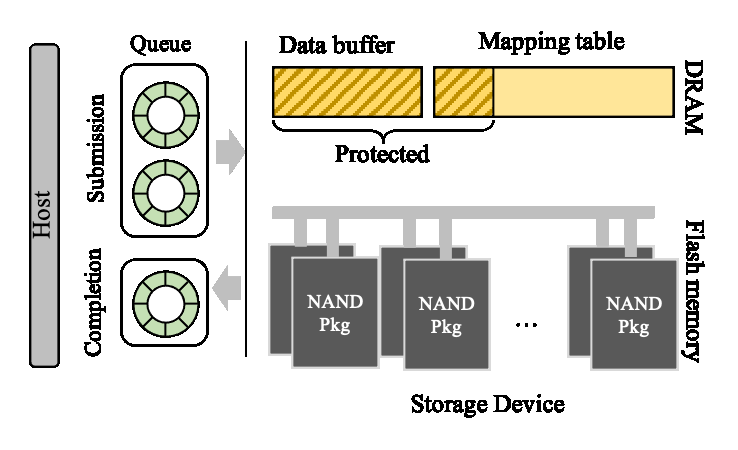
\includegraphics[width=0.4\textwidth]{figure/dawid_ssd_archi.eps}
    \caption{\textbf{Dawid-SSD}}
    \label{fig_dawid_archi}
\end{figure}


We implement \ours{} in \texttt{FEMU}, an open-source SSD development
framework~\cite{li2018case}. Fig.~\ref{fig_dawid_archi} shows the overall
architecture of \ours{}-SSD and its internal data structures. As the original
version of \texttt{FEMU} directly writes data to flash memories without write
buffering, we extend it to use a small-sized write buffer, which aggregates and  
batches user writes into the underlying flash memory.  

\ours{}-SSD maintains three different threads that are executing concrrently
within SSDs.  The \texttt{nvm\_poller} takes a charge of transferring requests
between NVMe queues and FTL-internal queues. The FTL-internal queue consists of
a pair of sub-queues, each of which is named \texttt{to\_ftl} and
\texttt{to\_poller}). This separation is intended to enable a non-blocking
access to queues by allowing only a single writer for each queue.  Second, the
\texttt{ftl\_thread} essentially handles the ingress requests from the internal
queues. For write, it transfers data from the host memory to the SSD-internal
write buffer with DMA and updates the associated entry in a translation page to
point to the write buffer. Then, it notifies the completion of request to the
\texttt{nvm\_poller} by enqueueing the acknowledgement into the
\texttt{to\_poller} queue.  Because \ours{} protects the entire space of write
buffer with capacitance, data persistency is guaranteed for all acknowledged
writes.  For read, the \texttt{ftl\_thread} retrieves the requested data by
consulting the mapping table and transfers it to the host. 

The \texttt{ftl\_flush\_thread} plays a role of writing data from a DRAM-buffer
into a flash memory.  With the \texttt{FIFO} policy, the user writes are issued
to NAND flash memory in the order they arrive into the buffer. However, \ours{}
flushes buffered writes in the order such that it least increases the dirty memory
footprint of the mapping table.  To realize this design, \ours{} maintains two
data structures, as depicted in Fig.~\ref{fig_dawid_archi}(b). First, \textit{a
zero-cost list} that holds the indexes to tranlsation pages that is already
in a dirty state, and second, \textit{a max binary heap} that
maintains the indexes to translation pages sorted by the number of buffered
user write requests associated with that page.  

%When there is sufficient bandwidth at underlying NAND flash subsystem for writes, 
When a half of the write buffer becomes occupied, flushing is invoked. \ours{}-SSD
first flushes user data whose translation pages in the zero-cost list, and then
persists user data as their translation pages are ordered by the max binary
heap. By doing so, each user write minimizes the number of eventual
translation page write, and each translation page write maximizes the number of
persisted mapping entries. These data structures are updated by the \texttt{ftl\_thread} 
when a write request arrives at SSD. 
To exploit the SSD internal parallelism, we send data to flash memory in
batches by the number of NAND flash chips that can be written simultaneously.

Once the write operations of NAND flash memory complete,
\texttt{ftl\_flush\_thread} updates the mapping table entries to point to the
physical address of the data in a flash memory.  At this moment, if the number
of dirty mapping table pages goes beyond the protectable number of pages,
\texttt{ftl\_flush\_thread} persists the mapping table page to flash memory.
This is also conducted in batches by the number of NAND flash chips that can be
written simultaneously.


\begin{figure*}[t]
    \centering{}
	\subfloat[Sequential] { 
	    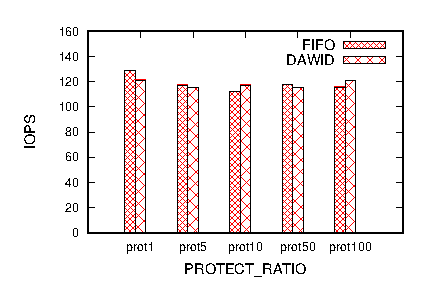
\includegraphics[width=0.3\textwidth]{expr/micro_220517/perf/SEQ/perf_SEQ.eps}
	} 
	\subfloat[Random] { 
	    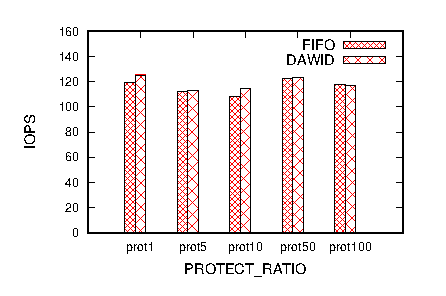
\includegraphics[width=0.3\textwidth]{expr/micro_220517/perf/RAND/perf_RAND.eps}
	} 
	\subfloat[JESD] { 
	    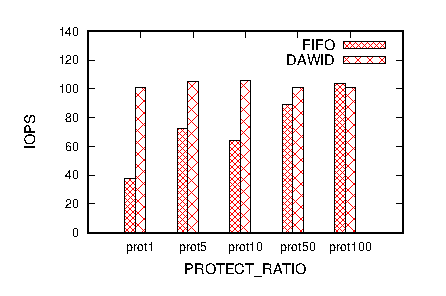
\includegraphics[width=0.3\textwidth]{expr/micro_220517/perf/JESD/perf_JESD.eps}
	}
    \caption{\textbf{IOPS}}
\end{figure*} 


\iffalse
\begin{figure*}[t]
	\includegraphics[width=0.9\textwidth]{expr/micro_220517/wt/result/total.rslt.eps}
    \caption{\textbf{Write Traffic}}
\end{figure*} 
\fi


\begin{figure*}[t]
    \centering{}
	\subfloat[Sequential] { 
	    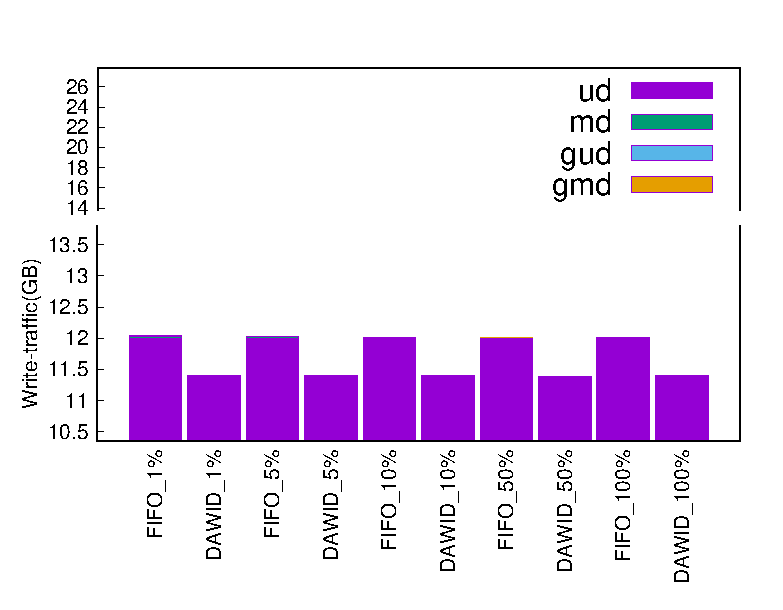
\includegraphics[width=0.3\textwidth]{expr/micro_220517/wt/result/SEQ.eps}
	} 
	\subfloat[Random] { 
	    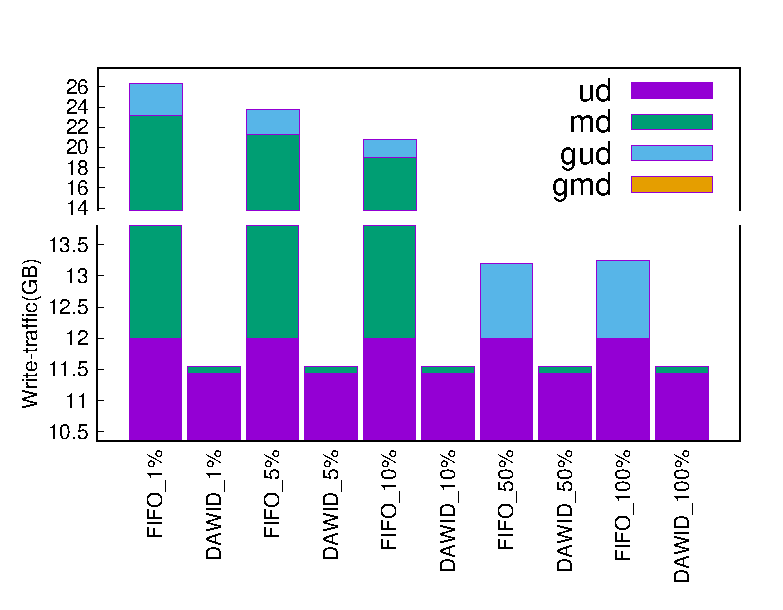
\includegraphics[width=0.3\textwidth]{expr/micro_220517/wt/result/RAND.eps}
	} 
	\subfloat[JESD] { 
	    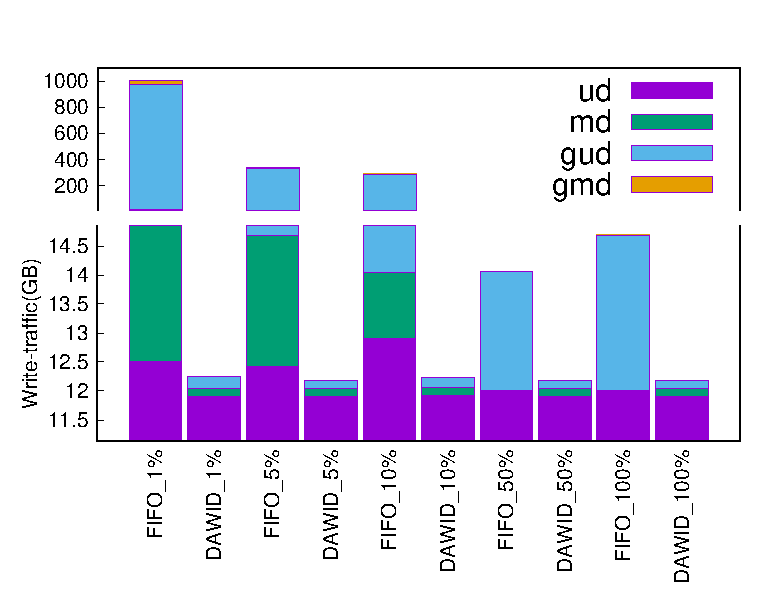
\includegraphics[width=0.3\textwidth]{expr/micro_220517/wt/result/JESD.eps}
	}
    \caption{\textbf{Write Traffic}}
\end{figure*} 


\iffalse
\begin{figure*}[t]
    \centering{}
	\subfloat[Sequential] { 
	    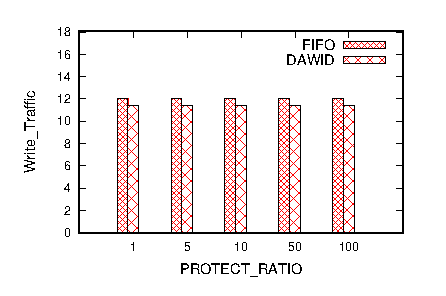
\includegraphics[width=0.3\textwidth]{expr/micro_220517/wt/perf_SEQ.eps}
	} 
	\subfloat[Random] { 
	    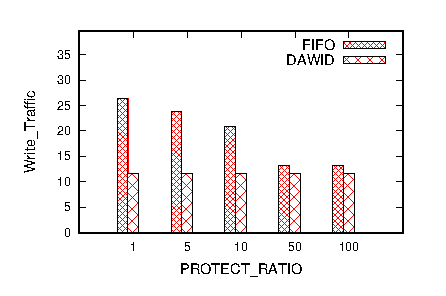
\includegraphics[width=0.3\textwidth]{expr/micro_220517/wt/perf_RAND.eps}
	} 
	\subfloat[JESD] { 
	    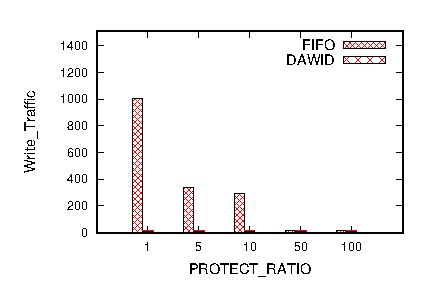
\includegraphics[width=0.3\textwidth]{expr/micro_220517/wt/perf_JESD.eps}
	}
    \caption{\textbf{Write Traffic}}
\end{figure*} 
\fi




\iffalse
%% CACHE_MISS
\begin{table}
    \centering
    \fontsize{11}{11}
    \begin{tabular}{| l | r | r | r | r | } %% KVS cache-ref cache-miss 
    \hline
    \footnotesize{\textbf{Workload}} & \footnotesize{\textbf{OPs}} & \footnotesize{\textbf{Footprint(Data)}} & \footnotesize{\textbf{Footprint(Index)}} \\ \hline \hline
    \footnotesize{sequential} & \footnotesize{2M} & \footnotesize{0,000} & \footnotesize{00,000} \\ \hline
    \footnotesize{random} & \footnotesize{2M} & \footnotesize{0,000} & \footnotesize{00,000} \\ \hline
    \footnotesize{webserver} & \footnotesize{2M} & \footnotesize{5.2G} & \footnotesize{5.8G} \\ \hline
    \footnotesize{fileserver} & \footnotesize{2M} & \footnotesize{1.9G} & \footnotesize{2.2G} \\ \hline
    \footnotesize{linkbench run} & \footnotesize{2M} & \footnotesize{5.0G} & \footnotesize{14.8G} \\ \hline
    \footnotesize{tpcc} & \footnotesize{2M} & \footnotesize{2.7G} & \footnotesize{5.8G} \\ \hline
%    \footnotesize{sequential} & \footnotesize{29,831} & \footnotesize{4,125} & \footnotesize{21,986} & \footnotesize{2,731} \\ \hline 
%    \footnotesize{random} & \footnotesize{38,272} & \footnotesize{5,810} & \footnotesize{20,949} & \footnotesize{2,727} \\ \hline 
%    \footnotesize{linkbench} & \footnotesize{9,238} & \footnotesize{4,368} & \footnotesize{4,844} & \footnotesize{1,938} \\ \hline 
%    \footnotesize{TPC-C} & \footnotesize{38,732} & \footnotesize{29,529} & \footnotesize{8,389} & \footnotesize{4,092} \\ \hline 
%    \footnotesize{Webserver} & \footnotesize{38,732} & \footnotesize{29,529} & \footnotesize{8,389} & \footnotesize{4,092} \\ \hline 
%    \footnotesize{Fileserver} & \footnotesize{38,732} & \footnotesize{29,529} & \footnotesize{8,389} & \footnotesize{4,092} \\ \hline 
    %\footnotesize{+overwrite} & \footnotesize{68,103} & \footnotesize{9,935} & \footnotesize{42,935} & \footnotesize{5,458} \\ \hline
    %\footnotesize{+readrandom} & \footnotesize{77,341} & \footnotesize{14,303} & \footnotesize{47,779} & \footnotesize{7,396} \\ \hline
    %\footnotesize{+seekrandom} & \footnotesize{116,073} & \footnotesize{43,832} & \footnotesize{56,168} & \footnotesize{11,488} \\ \hline
    \end{tabular}
    \vspace{5pt}
    \caption{\textbf{Number of cache references and misses.}
        \textbf{Ref(R)} is the number of cache references when running RocksDB; 
        \textbf{Miss(R)}, the number of cache misses with RocksDB; 
        \textbf{Ref(J)}, references with JFDB; and \textbf{Miss(J)}, misses with JFDB.
    }    
    \label{tab_cache_miss}
\end{table}
\fi 

\iffalse
\begin{figure*}[t]
    \centering{}
	\subfloat[Random Write] { 
	    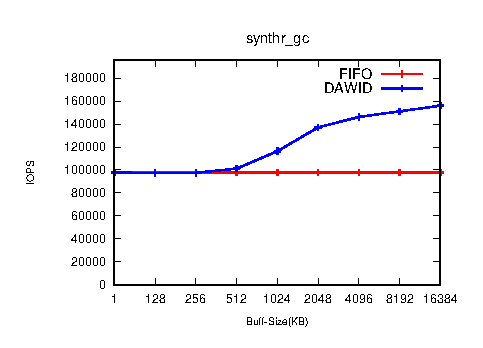
\includegraphics[width=0.3\textwidth]{expr/micro/synthr_gc.eps}
	} 
	\subfloat[Linkbench] { 
	    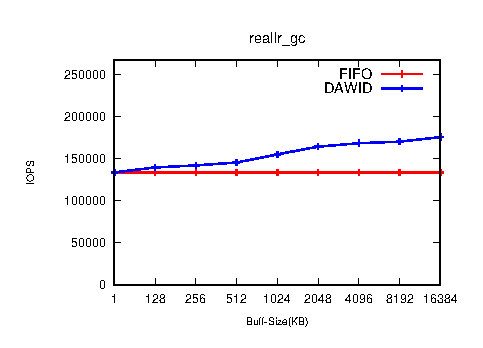
\includegraphics[width=0.3\textwidth]{expr/micro/reallr_gc.eps}
	} 
	\subfloat[TPCC] { 
	    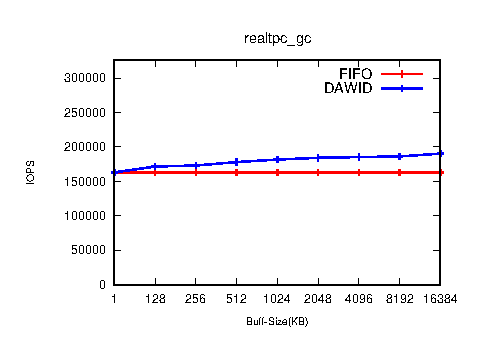
\includegraphics[width=0.3\textwidth]{expr/micro/realtpc_gc.eps}
	}
    \caption{\textbf{IOPS}}
\end{figure*} 



\begin{figure*}[t]
    \centering{}
	\subfloat[Filebench Webserver] { 
	    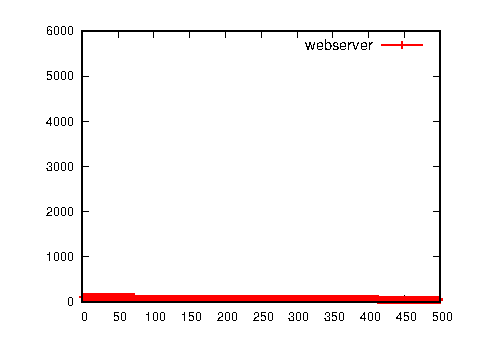
\includegraphics[width=0.4\textwidth]{webserver_uniq_500.eps}
	} 
	\subfloat[Filebench Fileserver] { 
	    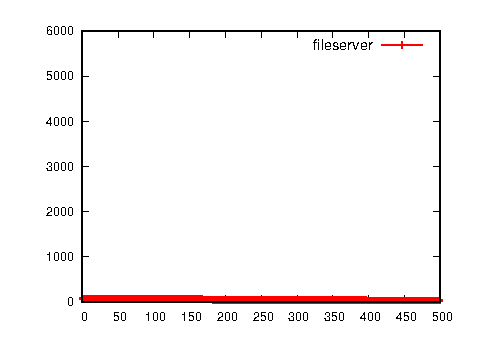
\includegraphics[width=0.4\textwidth]{fileserver_uniq_500.eps} 
	} 
    \caption{\textbf{Workload Characteristic.}}

    \centering{} 
	\subfloat[Linkbench Run] { 
	    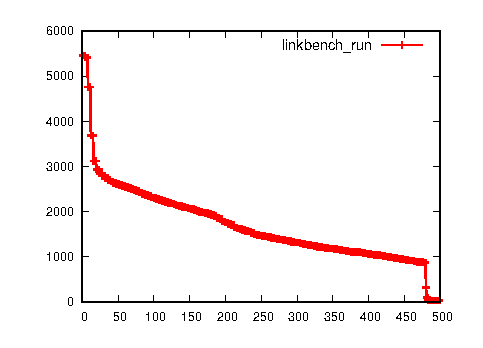
\includegraphics[width=0.4\textwidth]{linkbench_r_uniq_500.eps}
	} 
	\subfloat[TPCC] { 
	    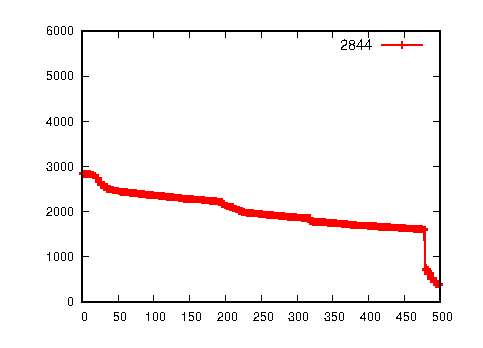
\includegraphics[width=0.4\textwidth]{tpcc_20_500.eps}
	}
    \caption{\textbf{Workload Characteristic.}}
\end{figure*} 

\fi

%\subsection{Performance results}
\section{Evaluation}
%We assume 1\% of the mapping table is protected via capacitors in a 64GB SSD. 
%The 64GB SSD is using DRAM and assumes that 1\% of the mapping table is
%protected. 
We measured the performance of \ours{} using fio benchmark~\cite{fio-bench},
running 4KB sequential writes, 4KB random writes, and the skewed read-write
mixed workload that follows JESD219 using 8 threads.  A total of 90GB of data
was written to the 30GB area.

\iffalse
\begin{table}[tb]
    \centering
    \fontsize{11}{11}
    \small
	% Model Manufacturer Category PLP-Support Capacitor 
    %\begin{tabular}{p{2.4cm}|p{1.3cm}|p{1.2cm}|l}
    %\begin{tabular}{p{2.4cm}|p{2.4cm}|p{2.4cm}|p{2.4cm}|p{2.4cm}}
    \begin{tabular}{|p{5cm}|l|}
        % \hline
        % \multirow{4}{*}{{\rotatebox{90}{\parbox{1.2cm}{\centering \footnotesize{Concurrency}}}}} 
		\hline
        \bf{Data Type} &  \bf{Size} \\ \hline \hline
        % \footnotesize{\bf{Ratio}} \\ \hline \hline
	    {User Data Buffer} & {4MB} \\ \hline
		{Mapping Table} & {512MB} \\ \hline
		{Mapping Table Directory} & {512KB} \\ \hline 
% 		\footnotesize{Mapping Table Directory} & \footnotesize{128KB} & \footnotesize{0.02}\% \\ \hline
		{Metadata for Allocation} & {1MB} \\ \hline 
		{Metadata for GC(Garbage Collection)} & {9MB}  \\ \hline 
		{Total Buffer Memory} & {526.5MB} \\ \hline
% 		\footnotesize{SSD Capacity} & \footnotesize{512GB} & -  \\ \hline
    \end{tabular}
    \caption{\textbf{Components of the SSD-internal buffer.}}
    \label{tab:ssd_buff_comp}
    \vspace{-10pt}
\end{table}
\fi

\iffalse
\begin{table}[tb]
    \centering
    \fontsize{11}{11}
    \small
	% Model Manufacturer Category PLP-Support Capacitor 
    %\begin{tabular}{p{2.4cm}|p{1.3cm}|p{1.2cm}|l}
    %\begin{tabular}{p{2.4cm}|p{2.4cm}|p{2.4cm}|p{2.4cm}|p{2.4cm}}
    \begin{tabular}{|p{5cm}|l|}
        % \hline
        % \multirow{4}{*}{{\rotatebox{90}{\parbox{1.2cm}{\centering \footnotesize{Concurrency}}}}} 
		\hline
		\bf{Configuration} & \bf{Size} \\ \hline \hline
        Channel & 8x \\ \hline
        Way & 4x \\ \hline
        Die & 4x \\ \hline
        Plane & 4x \\ \hline
        Page Size & 4KB \\ \hline
        SSD Capacity & 512GB \\ \hline
    \end{tabular}
    \caption{\textbf{SSD Configuration.}}
    \label{tab:ssd_config}
    % \vspace{-10pt}
\end{table}
\fi
